% COMMON RINGS
\newcommand{\N}{\mathbb{N}}
\newcommand{\R}{\mathbb{R}}
\newcommand{\Z}{\mathbb{Z}}
\newcommand{\T}{\mathbb{T}}
\renewcommand{\S}{\mathbb{S}}

% Common operations and functions
\newcommand{\gr}{\operatorname{gr}}
\newcommand{\id}{\operatorname{id}}

% Common sets
\newcommand{\singularknots}{\mathcal{K}^{\bullet}}

% Crossings and singularities
\newcommand*{\double}{\adjustbox{valign=c}{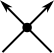
\includegraphics[width=0.05\textwidth]{graphics/glyph_singular_point.pdf}}}
\newcommand*{\poscross}{\adjustbox{valign=c}{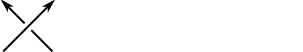
\includegraphics[width=0.05\textwidth]{graphics/glyph_positive_crossing.pdf}}}
\newcommand*{\negcross}{\adjustbox{valign=c}{\includegraphics[width=0.05\textwidth]{graphics/glyph_negative_crossing.pdf}}}
\newcommand*{\virtcross}{\adjustbox{valign=c}{\includegraphics[width=0.05\textwidth]{graphics/glyph_virtual_crossing.pdf}}}
\newcommand*{\semivirtposcross}{\adjustbox{valign=c}{\includegraphics[width=0.05\textwidth]{graphics/glyph_semivirtual_positive_crossing.pdf}}}
\newcommand*{\semivirtnegcross}{\adjustbox{valign=c}{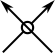
\includegraphics[width=0.05\textwidth]{graphics/glyph_semivirtual_negative_crossing.pdf}}}
\newcommand*{\uncross}{\adjustbox{valign=c}{\includegraphics[width=0.05\textwidth]{graphics/glyph_uncrossing.pdf}}}
\newcommand*{\unknot}{\adjustbox{valign=c}{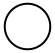
\includegraphics[width=0.05\textwidth]{graphics/glyph_unknot.pdf}}}

% T4T and T1T graphics
\newcommand*{\tftsouth}{\adjustbox{valign=c}{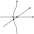
\includegraphics[width=0.11\textwidth]{topological_four_term_south.pdf}}}
\newcommand*{\tfteast}{\adjustbox{valign=c}{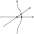
\includegraphics[width=0.11\textwidth]{topological_four_term_east.pdf}}}
\newcommand*{\tftnorth}{\adjustbox{valign=c}{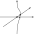
\includegraphics[width=0.11\textwidth]{topological_four_term_north.pdf}}}
\newcommand*{\tftwest}{\adjustbox{valign=c}{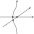
\includegraphics[width=0.11\textwidth]{topological_four_term_west.pdf}}}

\newcommand*{\topologicalonecotermgraphic}{\adjustbox{valign=c}{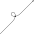
\includegraphics[width=0.11\textwidth]{topological_one_term.pdf}}}

% Typewriter tags for equation labels
\newcommand{\differentiability}{\texttt{DIFF}}
\newcommand{\differentiabilitystar}{\texttt{DIFF}\ensuremath{^\ast}}

\newcommand{\topologicalfourtermstar}{\texttt{T4T}\ensuremath{^\ast}}
\newcommand{\topologicalfourterm}{\texttt{T4T}}

\newcommand{\topologicalonetermstar}{\texttt{T1T}\ensuremath{^\ast}}
\newcommand{\topologicaloneterm}{\texttt{T1T}}

\newcommand{\fourtermstar}{\texttt{4T}\ensuremath{^\ast}}
\newcommand{\fourterm}{\texttt{4T}}

\newcommand{\onetermstar}{\texttt{1T}\ensuremath{^\ast}}
\newcommand{\oneterm}{\texttt{1T}}

\newcommand{\as}{\texttt{AS}}

\newcommand{\stu}{\texttt{STU}}

\newcommand{\ihx}{\texttt{IHX}}

\newcommand{\ronef}{\texttt{R1}\ensuremath{^{\texttt{f}}}}
\newcommand{\rtwo}{\texttt{R2}}
\newcommand{\rthree}{\texttt{R3}}

\newcommand{\vrone}{\texttt{VR1}}
\newcommand{\vrtwo}{\texttt{VR2}}
\newcommand{\vrthree}{\texttt{VR3}}
\newcommand{\vrfour}{\texttt{VR4}}

\newcommand{\oc}{\texttt{OC}}

\newcommand{\tc}{\texttt{TC}}


% Boldface tags for knot sums
\newcommand{\tftterm}{\mathbf{T4T}}
\newcommand{\totterm}{\mathbf{T1T}}

% 4T graphics
\newcommand*{\ftsouth}{\adjustbox{valign=c}{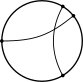
\includegraphics[width=0.11\textwidth]{four_term_south.pdf}}}
\newcommand*{\fteast}{\adjustbox{valign=c}{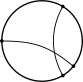
\includegraphics[width=0.11\textwidth]{four_term_east.pdf}}}
\newcommand*{\ftnorth}{\adjustbox{valign=c}{
\includegraphics[width=0.11\textwidth]{four_term_north.pdf}}}
\newcommand*{\ftwest}{\adjustbox{valign=c}{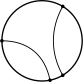
\includegraphics[width=0.11\textwidth]{four_term_west.pdf}}}

% 1T graphics
\newcommand*{\isolatedchord}{\adjustbox{valign=c}{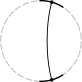
\includegraphics[width=0.11\textwidth]{one_term.pdf}}}

% Connected sum
\newcommand{\connect}{\mathbin{\sharp}}
